\chapter{Variable importances}\label{ch:importances}

\begin{remark}{Outline}
In this chapter, we study variable importance measures as computed from forests of
randomized trees. In Section~\ref{sec:6:importances}, we first present how
random forests can be used to assess the importance of input variables.  We
then derive in Section~\ref{sec:6:theory} a characterization in asymptotic
conditions and show that variable importances derived from totally randomized trees
offer a three-level decomposition of the information jointly  contained in the
input variables about the output. In Section~\ref{sec:6:variable-relevance}, we
show that this  characterization only depends on the relevant variables and
then discuss these ideas in Section~\ref{sec:6:variants} in the context of
variants closer to the Random Forest algorithm. Finally, we illustrate these
results on an artifical problem in Section~\ref{sec:6:illustration}.
\textit{This chapter is based on previous work published in \citep{louppe:2013}.}
\end{remark}

An important task in many scientific fields is the prediction of  a response
variable based on a set of predictor variables. In many situations though, the
aim is not only to make the most accurate predictions of the response but also
to identify which predictor variables are the most important to make these
predictions, e.g. in order to understand the underlying process. Because of
their applicability to a wide range of problems and their capability to
build accurate models and, at the same time, to provide variable importance
measures, random forests have become a major data analysis tool used with
success in various scientific areas.

Despite their extensive use in applied research, only a couple of works have
studied the theoretical properties and statistical mechanisms of these
algorithms. \citet{zhao:2000}, \citet{breiman:2004},
\citet{biau:2008,biau:2012}, \citet{meinshausen:2006} and \citet{lin:2006}
investigated simplified to very realistic variants of these algorithms and
proved  the consistency of those variants. Little is known however regarding
the variable importances computed by random forests, and -- as far as we know
-- the work of~\citet{ishwaran:2007} is indeed the only theoretical study of
tree-based variable importance measures. In this chapter, we aim at filling
this gap and present a theoretical  analysis of the Mean Decrease Impurity
importance derived from ensembles of randomized trees.



% A forest of trees is impenetrable
% as far as simple interpretations of its mechanims go~\citep{breiman:2001}.


\section{Variable importances}
\label{sec:6:importances}

\subsection{Importances in single decision trees}

In the context of single decision trees, \cite{breiman:1984} first defined
the measure of importance of a variable $X_j$ as
\begin{equation}
\text{Imp}(X_j) = \sum_{t\in \varphi} \Delta I(\tilde{s}^j_t, t),
\end{equation}
where $\tilde{s}^j_t$ is the best \textit{surrogate split}
for $s_t$, that is the closest split defined on variable $X_j$ that can mimic the actual
split $s_t$ defined at node $t$. The use of surrogate splits was proposed to
account for masking effects: it may indeed happen that some variable $X_{j_2}$
never occurs in any split because it leads to splits that are slightly worse,
and therefore not selected, than those of some other variable $X_{j_1}$.
However, if $X_{j_1}$ is removed and another tree is grown, $X_{j_2}$ may now
occur prominently within the splits and the resulting tree may be nearly as good
as the original tree. In such a case, a relevant measure should detect the
importance of $X_{j_2}$. Accordingly, if $X_{j_2}$ is being masked at $t$ by
$X_{j_1}$ (i.e., if $X_{j_1}$ is used to split $t$), but if $\tilde{s}^{j_2}_t$ is similar to
$s_t$, but not quite as good, then $\Delta I(\tilde{s}^{j_2}_t, t)$ will be
nearly as large as $\Delta I(s_t, t)$ and therefore the proposed measure will
indeed account for the importance of $X_{j_2}$.

Thanks to randomization, masking effects are dampened within forests of
randomized trees. Even if $X_{j_2}$ is being masked by $X_{j_1}$ there is indeed
still a chance for $X_{j_2}$ to be chosen as a split if $X_{j_1}$ is not
selected among the $K$ variables chosen at random. Depending on the value $K$,
masking effects do not disappear entirely though. The use of bootstrap samples
also helps reduce masking effects, making $X_{j_1}$ or $X_{j_2}$ just slightly
better than the other due to the variations in the bootstrap samples.

\subsection{Importances in forests}

In the context of ensembles of randomized trees,
\cite{breiman:2001,breiman:2002} proposed to evaluate the importance of
a variable $X_j$  for predicting  $Y$ by adding up the weighted impurity decreases $p(t) \Delta
i(s_t, t)$ for all nodes $t$ where $X_j$ is used, averaged over all trees $\varphi_m$ (for $m=1,\dots,M$)
in the forest:
\begin{equation}\label{eq:mdi}
\text{Imp}(X_j) = \frac{1}{M} \sum_{m=1}^M \sum_{t \in \varphi_{m}} 1(j_t = j) \Big[ p(t) \Delta i(s_t, t) \Big],
\end{equation}
where $p(t)$ is the proportion $\tfrac{N_t}{N}$ of samples
reaching $t$ and where $j_t$ denotes the identifier of the variable used for splitting node $t$. When
using the Gini index as impurity function, this measure is known as the
\textit{Gini importance} or \textit{Mean Decrease Gini}. However, since it can
be defined for any impurity measure $i(t)$, we will refer to Equation~\ref{eq:mdi}
as the \textit{Mean Decrease Impurity} importance (MDI), no matter the impurity
measure $i(t)$. We will characterize and derive results for this measure in the
rest of this text.

In addition to MDI, \cite{breiman:2001,breiman:2002} also proposed to evaluate
the importance of a variable $X_j$ by measuring the \textit{Mean Decrease
Accuracy} (MDA) or, equivalently, by measuring the \textit{Mean Increase Error},
of the forest when the values of $X_j$ are randomly permuted in the out-of-bag
samples. For that reason, this latter measure is also known as the
\textit{permutation importance}. Formally, in regression, the permutation
importance of $X_j$ is given as:
\begin{align}\label{eq:mda}
\text{Imp}(X_j) &=  \mathbb{E}_{\pi_j} \Bigg\{ \frac{1}{N} \sum_{(\mathbf{x}_i^\prime,y_i) \in \pi_j({\cal L})} L(\frac{1}{M^{-i}} \sum_{l=1}^{M^{-i}} \varphi_{{\cal L}^{m_{k_l}}}(\mathbf{x}_i^\prime), y_i) \Bigg\} \nonumber  \\
&\hookrightarrow - \frac{1}{N} \sum_{(\mathbf{x}_i,y_i) \in {\cal L}} L(\frac{1}{M^{-i}} \sum_{l=1}^{M^{-i}} \varphi_{{\cal L}^{m_{k_l}}}(\mathbf{x}_i), y_i)
\end{align}
where $\pi_j({\cal L})$ denotes a replicate of ${\cal L}$ in which in the
values of $X_j$ have been randomly permuted, and where
$m_{k_1},\dots,m_{k_{M^{-i}}}$ denote the indices of the trees that have been
built from bootstrap replicates that do not include $(\mathbf{x}_i, y_i)$. For
classification, the permutation importance is derived similarly as in
Equation~\ref{eq:mda}, except  that the out-of-bag average predictions are
replaced with the class which is the most likely, as computed from the out-of-bag
class probability estimates. Its rationale is that randomly permuting the
input variable $X_j$ should break its association with the response $Y$.
Therefore, if $X_j$ is in fact associated to $Y$, permuting its values should
also result in a substantial increase of error, as here measured by the
difference between the out-of-bag estimates of the generalization error. That
is, the larger the increase of error, the more important the variable, and
vice-versa.

Thanks to popular machine learning
softwares~\citep{breiman:2002,liaw:2002,pedregosa:2011},
both of these variable importance measures have shown their practical utility in
an increasing number of experimental studies. Little is known however regarding
their inner workings. \cite{strobl:2007b} compare both MDI and MDA and show
experimentally that the former is biased towards some predictor variables. As
explained by~\cite{white:1994} in case of single decision trees, this
bias stems from an unfair advantage given by the usual impurity functions $i(t)$
towards predictors with a large number of values. \cite{strobl:2008}
later showed  that MDA is biased as well, and that it overestimates the
importance of correlated variables -- although this effect was not confirmed in
a later experimental study by~\cite{genuer:2010}.  From a theoretical
point of view, \cite{ishwaran:2007} provides a detailed theoretical
development of a simplified version of MDA, giving key insights for the
understanding of the actual MDA.

\section{Theoretical study}
\label{sec:6:theory}

\subsection{Background}

To be self-contained, we first recall several definitions from information
theory (see \citep{cover:2012}, for further properties).

We suppose that we are given a probability space $(\Omega, {\cal E},
\mathbb{P})$ and  consider random variables defined on it taking a finite
number of possible values. We use upper case letters to denote such random
variables (e.g. $X, Y, Z, W \ldots$)  and calligraphic letters (e.g. $\cal X,
Y, Z, W \ldots$) to denote their image sets (of finite cardinality), and lower
case letters (e.g. $x, y, z, w \ldots$) to denote one of their possible values.
For a (finite) set of (finite) random variables $ X = \{X_{1}, \ldots ,
X_{p}\}$, we denote by $P_{X}(\mathbf{x}) = P_{X}(x_{1}, \ldots , x_{p})$ the
probability $\mathbb{P}(\{ \omega \in \Omega \mid  \forall j : 1, \ldots, p:
X_j(\omega) =x_j\})$, and by ${\cal X} = {\cal X}_{1} \times \cdots
\times {\cal X}_{p}$ the set of joint configurations of these random variables.
Given two sets of random variables, $X = \{X_{1}, \ldots , X_{p}\}$ and
$Y=\{Y_{1}, \ldots , Y_{q}\}$, we denote by $P_{X \mid Y}(\mathbf{x} \mid \mathbf{y}) = {P_{X, Y}
(\mathbf{x},  \mathbf{y})}/ {P_{Y}(\mathbf{y})}$ the conditional density of $X$ with respect to
$Y$.\footnote{To avoid problems, we suppose that all probabilities are strictly
positive, without fundamental limitation.}

With these notations, the joint (Shannon) entropy of a set of random variables
$X =\{X_{1}, \ldots , X_{p}\}$ is thus defined by
\begin{equation}
H(X)  = - \sum_{\mathbf{x} \in {\cal X}}P_{X} (\mathbf{x})\log_{2}P_{X}(\mathbf{x}),
\end{equation}
while the mean conditional entropy of a set of random variables $X = \{X_{1},
\ldots , X_{p}\}$, given the values of another set of random variables
$Y=\{Y_{1}, \ldots , Y_{q}\}$ is defined by
\begin{equation}
H(X\mid Y) = - \sum_{\mathbf{x} \in {\cal X}} \sum_{\mathbf{y} \in {\cal Y}} P_{X, Y} (\mathbf{x}, \mathbf{y}) \log_{2} P_{X \mid Y} (\mathbf{x} \mid \mathbf{y}).
 \end{equation}
The mutual information among the set of random variables $X =\{X_{1}, \ldots ,
X_{p}\}$ and the set of random variables $Y=\{Y_{1}, \ldots , Y_{q}\}$ is
defined by
 \begin{align}
 I(X; Y) &= - \sum_{\mathbf{x} \in {\cal X}} \sum_{\mathbf{y} \in {\cal Y}} P_{X, Y} (\mathbf{x}, \mathbf{y}) \log_{2} \frac{P_{X}(\mathbf{x}) P_{Y}(\mathbf{y})}{P_{X,Y}(\mathbf{x},\mathbf{y})} \\
 &= H(X) - H(X \mid Y) \nonumber \\
 &=  H(Y) - H(Y \mid X) \nonumber
 \end{align}

The mean conditional mutual information among the set of random variables $X
=\{X_{1}, \ldots , X_{p}\}$ and the set of random variables $Y=\{Y_{1}, \ldots
, Y_{q}\}$, given the values of a third set of random variables $Z=\{Z_{1},
\ldots , Z_{r}\}$, is defined by
 \begin{align}
 I(X; Y \mid Z) &= H(X \mid Z) - H(X \mid Y, Z)\\
 & = H(Y \mid Z) - H(Y \mid X, Z) \nonumber\\
& = - \sum_{\mathbf{x} \in {\cal X}} \sum_{\mathbf{y} \in {\cal Y}} \sum_{\mathbf{z} \in {\cal Z}} P_{X, Y, Z} (\mathbf{x}, \mathbf{y}, \mathbf{z}) \log_{2} \frac{P_{X \mid Z}(\mathbf{x} \mid \mathbf{z}) P_{Y\mid Z}(\mathbf{y} \mid \mathbf{z})}{P_{X,Y \mid Z}(\mathbf{x},\mathbf{y} \mid \mathbf{z})}\nonumber
\end{align}

We also recall the chaining rule
\begin{equation}
I(X, Z ; Y \mid W ) = I(X; Y \mid W  ) + I( Z ; Y \mid W, X),
\end{equation}
and the symmetry of the (conditional) mutual information among sets of random variables
\begin{equation}
I(X ; Y \mid Z) = I(Y ;  X  \mid Z).
\end{equation}


\subsection{Asymptotic analysis}

Let us now consider the MDI  importance as defined by Equation~\ref{eq:mdi},
and let us assume a set $V= \{X_1, ..., X_p\}$  of {\em categorical} input
variables and a {\em categorical} output $Y$. For the sake of simplicity we
will  use the Shannon entropy as impurity measure, and focus on totally
randomized trees; later on we will discuss other impurity measures and tree
construction algorithms.

Given a training sample ${\cal L}$ of $N$ joint observations of $X_1, ..., X_p,
Y$ independently drawn from the joint distribution $P(X_1, ..., X_p, Y)$, let us
assume that we infer from it an infinitely large ensemble of \textit{totally
randomized and fully developed trees}. In this setting, a totally randomized and
fully developed tree is defined as a decision tree in which each node $t$ is
partitioned using a variable $X_j$ picked uniformly at random among those not
yet used at the parent nodes of $t$, and where each $t$ is split into $|{\cal
X}_j|$ sub-trees, i.e., one for each possible value of ${\cal X}_j$, and where
the recursive construction process halts only when all $p$ variables have been
used along the current branch.  Hence, in such a tree, leaves are all at the
same depth $p$, and the set of leaves of a fully developed tree is in bijection
with the set $\cal X$ of all possible joint configurations of the $p$ input
variables. For example, if the input variables are all binary, the resulting
tree will have exactly $2^{p}$ leaves.

\begin{theorem}\label{thm:imp}
The MDI importance of $X_j \in V$ for $Y$ as computed
with an   infinite ensemble of fully developed totally randomized trees and an
infinitely large training sample is:
  \begin{equation}\label{eqn:imp-full}
  \text{Imp}(X_j)=\sum_{k=0}^{p-1} \frac{1}{C_p^k} \frac{1}{p-k} \sum_{B \in {\cal P}_k(V^{-j})} I(X_j;Y|B),
  \end{equation}
\end{theorem}
\noindent where $V^{-j}$ denotes the subset $V \setminus \{X_j\}$, ${\cal
P}_k(V^{-j})$ is the set of subsets of  $V^{-j}$ of cardinality $k$, and
$I(X_j;Y|B)$ is the conditional mutual information of $X_{j}$ and $Y$ given the
variables in $B$.

\begin{proof}
By expanding $\Delta i(s, t) = i(t) - p_L i(t_L) - p_R i(t_R)$ into
Equation~\ref{eq:mdi} and using the entropy $H(Y|t) = -\sum_j p(j|t) \log_2(p(j|t))$
as impurity measure $i(t)$, Equation~\ref{eq:mdi} can be rewritten in terms of
mutual information:
\begin{equation}
\text{Imp}(X_j) = \frac{1}{M} \sum_{m=1}^M \sum_{t \in \varphi_m} 1(j_t = j) p(t) I(Y;X_j|t)
\end{equation}

As the size $N$ of the training sample grows to infinity, $p(t)$ becomes the
(exact) probability (according to $P(X_1,\ldots,X_p,Y)$) that an object reaches
node $t$, i.e., a probability $P(B(t)=b(t))$ where $B(t)=(X_{i_1}, ...,
X_{i_{k}})$ is the subset of $k$ variables tested in the branch from the root
node to the parent of $t$ and $b(t)$ is the vector of values of these
variables. As the the number $M$ of totally randomized trees also grows to
infinity, the importance of a variable $X_j$ can then be written:
\begin{equation}
\text{Imp}(X_j)=\sum_{B\subseteq V^{-j}} \sum_{b\in {\cal X}_{i_1}\times ... \times {\cal X}_{i_{k}} } \alpha(B,b,X_j,p) P(B=b) I(Y;X_j|B=b),
\end{equation}
where $b$ is a set of values for the variables in $B$ and $\alpha(B,b,X_j,p)$ is
the probability that a node $t$ (at depth $k$) in a totally randomized tree
tests the variable $X_j$ and is such that $B(t)=B$ and $b(t)=b$.

Let us compute $\alpha(B,b,X_j,p)$. First, let us consider the probability that
a node $t$ tests the variable $X_j$ and is such that the branch leading to $t$
follows a path defined, in that particular order, by all $k$ variables $X_{i_1},
..., X_{i_{k}} \in B$ and their corresponding values in $b$. The probability of
that branch is the probability of picking (uniformly at random)  $X_{i_1}$  at
the root node times the probability of testing, in that order, the remaining
$X_{i_2}, ..., X_{i_{k}}$ variables in the sub-tree corresponding to the value
$x_{i_1}$ of $X_{i_1}$ defined in $b$. Note that, by construction, it is certain
that this particular sub-tree exists since the root node is split into $|{\cal
X}_{i_1}|$ sub-trees.  Then, the
probability of testing $X_j$ at the end of this branch is the probability of
picking $X_j$ among the remaining $p-k$ variables. By recursion, we thus have:
\begin{equation}
\frac{1}{p} \frac{1}{p-1} ... \frac{1}{p-k+1} \frac{1}{p-k} = \frac{(p-k)!}{p!} \frac{1}{p-k}
\end{equation}

Since the order along which the variables appear in the branch is of no
importance, $\alpha(B,b,X_j,p)$ actually includes all $k!$ equiprobable ways of
building a branch composed of the variables and values in $B$ and $b$. Then,
since a tree may at most contain a single such branch, whatever the order of the
tests, the probabilities may be added up and it comes:
\begin{equation}
\alpha(B,b,X_j,p)=k! \frac{(p-k)!}{p!} \frac{1}{p-k} = \frac{1}{C_p^k} \frac{1}{p-k}
\end{equation}

From the above expression, it appears that $\alpha(B,b,X_j,p)$ depends only on
the size $k$ of $B$ and on the number $p$ of variables. As such, by grouping in
the previous equation of $\text{Imp}(X_j)$ conditioning variable subsets $B$ according
to their sizes and using the definition of conditional mutual information,
$\alpha$ can be factored out, hence leading to the form foretold by Theorem~\ref{thm:imp}:
\begin{equation}
\text{Imp}(X_j)=\sum_{k=0}^{p-1} \frac{1}{C^k_p} \frac{1}{p-k} \sum_{B \in {\cal P}_k(V^{-j})} I(X_j;Y|B).
\end{equation}
\end{proof}

\begin{theorem}\label{thm:sum-of-imp}
For any ensemble of fully developed trees in asymptotic learning sample size
conditions (e.g., in the same conditions as those of Theorem~\ref{thm:imp}), we
have that
\begin{equation}\label{eqn:sum-of-imp}
\sum_{j=1}^{p} \text{Imp}(X_j) = I(X_{1}, \ldots, X_{p} ; Y).
\end{equation}
\end{theorem}

\begin{proof}
For any tree $\varphi$, we have that the sum of all importances estimated by
using an infinitely large sample $\cal L$ (or equivalently, by assuming perfect
knowledge of the joint distribution $P(X_1, ..., X_p, Y)$) is equal to $H(Y) -
\sum_{t \in \widetilde{\varphi}} p(t) H(Y|b(t))$, where $\widetilde{\varphi}$
denotes the set of all leaves of $\varphi$, and where $b(t)$  denotes the joint
configuration of all input variables leading to leaf $t$. This is true because
the impurities of all test nodes intervening in the computation of the variable
importances, except the impurity $H(Y)$ at the root node of the tree, cancel
each other when summing up the importances.

Since, when the tree is fully developed, $\sum_{t \in \widetilde{\varphi}} p(t)
H(Y|b(t))$ is obviously equal to the mean conditional entropy $H(Y | X_{1},
\ldots, X_{p})$ of $Y$ given all input variables, this implies that for any
fully developed tree we have that the sum of variable importances is equal to
$I(X_{1}, \ldots, X_{p} ; Y)$, and so this relation also holds when averaging
over an infinite ensemble of totally randomized trees.
\end{proof}

Together, theorems \ref{thm:imp} and \ref{thm:sum-of-imp} show that  variable
importances derived from totally randomized trees in asymptotic conditions
provide a three-level decomposition of the information $I(X_{1}, \ldots, X_{p}
; Y)$ contained in the set of input variables about the output variable. The
first level is a decomposition among input variables (see Equation~\ref{eqn:sum-of-imp}
of Theorem~\ref{thm:sum-of-imp}),  the second level is a
decomposition along the degrees $k$ of interaction terms of a variable with the
other ones (see the outer sum in Equation~\ref{eqn:imp-full} of
Theorem~\ref{thm:imp}), and the third level is a decomposition along the
combinations $B$ of interaction terms of fixed size $k$ of possible interacting
variables (see the inner sum in Equation~\ref{eqn:imp-full}).

We observe that the decomposition includes, for each variable, each and every
interaction term of each and every degree weighted in a fashion resulting only
from the combinatorics of possible interaction terms. In particular, since all
$I(X_j;Y|B)$ terms are at most equal to $H(Y)$, the prior entropy of $Y$,  the
$p$ terms of the outer sum of Equation~\ref{eqn:imp-full} are each upper
bounded by
\begin{equation}
\frac{1}{C^k_p}\frac{1}{p-k}\sum_{B \in {\cal P}_k(V^{-j})}
H(Y)=\frac{1}{C^k_p} \frac{1}{p-k} {C^k_{p-1}} H(Y) = \frac{1}{p}H(Y).
\end{equation}
As such,
the second level decomposition resulting from totally randomized trees makes the
$p$ sub-importance terms
\begin{equation}
\frac{1}{C^k_p} \frac{1}{p-k} \sum_{B \in {\cal P}_k(V^{-j})} I(X_j;Y|B)
\end{equation}
to equally contribute (at most) to the total
importance, even though they each include a combinatorially different number of
terms.


\section{Relevance of variables}
\label{sec:6:variable-relevance}

Following~\citet{kohavi:1997}, let us define as {\em relevant to $Y$ with
respect to $V$} a variable $X_j$ for which there exists at least one subset $B
\subseteq V$ (possibly empty) such that $I(X_j;Y|B)>0$. Thus we define as {\em
irrelevant to $Y$ with respect to $V$} a variable $X_i$ for which, for all $B
\subseteq V$, $I(X_i; Y|B)=0$. Remark that if $X_i$ is irrelevant to $Y$ with
respect to $V$, then by definition it is also irrelevant to $Y$ with respect to
any subset of $V$. However, if $X_j$ is relevant to $Y$ with respect to $V$,
then it is not necessarily relevant to $Y$ with respect to all  subsets of $V$.
Among the relevant variables, we also distinguish the {\em marginally} relevant
ones, for which $I(X_{j}; Y) > 0$, the  {\em strongly} relevant ones, for which
$I(X_{j}; Y | V^{-j}) > 0$,  and the {\em weakly} relevant variables, which are
relevant but not strongly relevant.

\begin{theorem}\label{thm:irrelevant}
  $X_i \in V$ is irrelevant to $Y$ with respect to $V$ if and only if  its
  infinite sample size importance as computed with an infinite ensemble of fully
  developed totally randomized trees built on $V$ for $Y$ is 0.
\end{theorem}

\begin{proof}
The proof directly results from the definition of irrelevance. If $X_i$ is
irrelevant with respect to $V$, then $I(X_i;Y|B)$ is zero for all $B \subseteq
V^{-i} \subset V$ and Equation~\ref{eqn:imp-full} reduces to $0$. Also, since
$I(X_i;Y|B)$ is non-negative for any $B$, $\text{Imp}(X_i)$ is zero if and only if all
its $I(X_i;Y|B)$ terms are zero. Since $\text{Imp}(X_i)$ includes all $I(X_i;Y|B)$
terms for $B \subseteq V^{-i}$, and since all of them are therefore null if
$\text{Imp}(X_i)=0$,  $X_i$ is thus, by definition, irrelevant with respect to
$V^{-i}$. $X_i$ is then also trivially irrelevant with respect to $V=V^{-i} \cup
\{X_i\}$ since $I(X_i;Y|B\cup\{X_i\})=0$ for any $B$.
\end{proof}

\begin{lemma}\label{lemma:adding-irrelevant}
  Let $X_i \notin V$ be an irrelevant variable for $Y$ with respect to $V$. The infinite
  sample size importance of $X_j \in V$ as computed with an infinite
  ensemble of fully developed totally randomized trees built on $V$ for $Y$ is the
  same as the importance derived when using $V\cup \{X_i\}$ to build the ensemble of trees for $Y$.
\end{lemma}

\begin{proof}
Let $X_i \notin V$ be an irrelevant variable with respect to $V$. For $X_j \in
V$, $B \subseteq V^{-j}$, using the chain rules of mutual information, we have:
\begin{align}
I(X_j, X_i;Y|B) &= I(X_j;Y|B) + I(X_i;Y|B \cup \{X_j\})  \\
                &= I(X_i;Y|B) + I(X_j;Y|B \cup \{X_i\})
\end{align}
If $X_i$ is irrelevant with respect to $V$, i.e., such that $I(X_i;Y|B)=0$ for
all $B\subseteq V$, then $I(X_i;Y|B \cup \{X_j\})$ and $I(X_i;Y|B)$ both equal
$0$, leading to
\begin{equation}
I(X_j;Y|B \cup \{X_i\}) = I(X_j;Y|B)
\end{equation}

Then, from Theorem~\ref{thm:imp}, the importance of $X_j$ as computed with an
infinite ensemble of totally randomized trees built on $V\cup \{X_i\}$ can be
simplified to:
\begin{align}
  \text{Imp}(X_j)&=\sum_{k=0}^{p-1+1} \frac{1}{C_{p+1}^k} \frac{1}{p+1-k} \sum_{B \in {\cal P}_k(V^{-j} \cup \{X_i\})} I(X_j;Y|B)\nonumber\\
          &=\sum_{k=0}^{p} \frac{1}{C_{p+1}^k} \frac{1}{p+1-k} \left[ \sum_{B \in {\cal P}_k(V^{-j})} I(X_j;Y|B) + \sum_{B \in {\cal P}_{k-1}(V^{-j})} I(X_j;Y|B \cup \{X_i\})  \right] \nonumber\\
          &=\sum_{k=0}^{p-1} \frac{1}{C_{p+1}^k} \frac{1}{p+1-k} \sum_{B \in {\cal P}_k(V^{-j})} I(X_j;Y|B) + \nonumber\\
          & \hookrightarrow \sum_{k=1}^{p} \frac{1}{C_{p+1}^k} \frac{1}{p+1-k} \sum_{B \in {\cal P}_{k-1}(V^{-j})} I(X_j;Y|B)\nonumber\\
          &=\sum_{k=0}^{p-1} \frac{1}{C_{p+1}^k} \frac{1}{p+1-k} \sum_{B \in {\cal P}_k(V^{-j})} I(X_j;Y|B) + \nonumber\\
          & \hookrightarrow \sum_{k'=0}^{p-1} \frac{1}{C_{p+1}^{k'+1}} \frac{1}{p+1-k'-1} \sum_{B \in {\cal P}_{k'}(V^{-j})} I(X_j;Y|B)\nonumber\\
          &=\sum_{k=0}^{p-1} \left[ \frac{1}{C_{p+1}^k} \frac{1}{p+1-k} + \frac{1}{C_{p+1}^{k+1}} \frac{1}{p-k} \right] \sum_{B \in {\cal P}_k(V^{-j})} I(X_j;Y|B)\nonumber\\
          &=\sum_{k=0}^{p-1} \frac{1}{C^k_p} \frac{1}{p-k} \sum_{B \in {\cal P}_k(V^{-j})} I(X_j;Y|B)
\end{align}
The last line above exactly corresponds to the importance of $X_j$ as computed
with an infinite ensemble of totally randomized trees built on $V$, which proves
Lemma~\ref{lemma:adding-irrelevant}.
\end{proof}

\begin{theorem}\label{thm:relevant}
  Let $V_R \subseteq V$ be the subset of all variables in $V$ that are relevant to $Y$ with
  respect to $V$. The infinite sample size importance of any variable $X_j \in
  V_R$ as computed with an infinite ensemble of fully developed totally randomized
  trees built on $V_R$ for $Y$ is the same as its importance computed in the same conditions by using all variables in $V$. That is:
    \begin{align}
      \text{Imp}(X_j)&=\sum_{k=0}^{p-1} \frac{1}{C_p^k} \frac{1}{p-k} \sum_{B \in {\cal P}_k(V^{-j})} I(X_j;Y|B)\nonumber \\
                     &=\sum_{l=0}^{r-1} \frac{1}{C_r^l} \frac{1}{r-l} \sum_{B \in {\cal P}_l(V_R^{-j})} I(X_j;Y|B)
    \end{align}
  where $r$ is the number of relevant variables in $V_R$.
\end{theorem}

\begin{proof}
Let us assume that $V_R$ contains $r \leq p$ relevant variables. If an infinite
ensemble of totally randomized trees were to be built directly on those $r$
variables then, from Theorem~\ref{thm:imp}, the importance of a relevant
variable $X_j$ would be:
\begin{equation}%\label{eqn:imp-rel}
  \text{Imp}(X_j)=\sum_{l=0}^{r-1} \frac{1}{C_r^l} \frac{1}{r-l} \sum_{B \in {\cal P}_l(V_R^{-m})} I(X_j;Y|B)
\end{equation}

Let $X_i \in V \setminus V_R$ be one of the $p-r$ irrelevant variables in $V$
with respect to $V$. Since $X_i$ is also irrelevant with respect to $V_R$, using
Lemma~\ref{lemma:adding-irrelevant}, the importance of $X_j$ when the ensemble
is built on $V_R \cup \{X_i\}$ is the same as the one computed on $V_R$ only
(i.e., as computed by the equation above). Using the same argument,
adding a second irrelevant variable $X_{i'}$ with respect to $V$ -- and therefore
also with respect to $V_R \cup \{X_i\}$ -- and building an ensemble of totally
randomized trees on $V_R \cup \{X_i\} \cup \{X_{i'}\}$ will yield importances
that are the same as those computed on $V_R \cup \{X_i\}$, which are themselves
the same as those computed by an ensemble built on $V_R$. By induction, adding
all $p-r$ irrelevant variables has therefore no effect on the importance of
$X_j$, which means that:
\begin{align}%\label{eqn:imp-rel-equiv}
  \text{Imp}(X_j)&=\sum_{k=0}^{p-1} \frac{1}{C_p^k} \frac{1}{p-k} \sum_{B \in {\cal P}_k(V^{-j})} I(X_j;Y|B)\nonumber \\
          &=\sum_{l=0}^{r-1} \frac{1}{C_r^l} \frac{1}{r-l} \sum_{B \in {\cal P}_l(V_R^{-m})} I(X_j;Y|B)
\end{align}
\end{proof}

Theorems~\ref{thm:irrelevant} and \ref{thm:relevant} show that the
importances computed with an ensemble of totally randomized trees depends only
on the relevant variables. Irrelevant variables have a zero importance and do
not affect the importance of relevant variables. Practically, we believe that
such properties are desirable conditions for a sound criterion assessing the
importance of a variable. Indeed, noise should not be credited of any importance
and should not make any other variable more (or less) important.

Intuitively, the independence with respect to irrelevant variables can be partly
attributed to the fact that splitting at $t$ on some irrelevant variable $X_i$
should only dillute the local importance $p(t) \Delta i(t)$ of a relevant
variable $X_j$ into the children $t_L$ and $t_R$, but not affect the total sum.
For instance, if $X_j$ was to be used at $t$, then the local importance would be
proportional to $p(t)$. By contrast, if $X_i$ was to be used at $t$ and $X_j$ at
$t_L$ and $t_R$, then the sum of the local importances for $X_j$ would be
proportional to $p(t_L) + p(t_R)=p(t)$, which does not change anything.
Similarly, one can recursively invoke the same argument if $X_j$ was to be used
deeper in $t_L$ or $t_R$.

A second reason comes from the
fact that local importances are collected only in nodes $t$ where $X_j$ is used.
By contrast, if local importances were summed over all nodes (e.g., using
surrogate splits), then it would necessarily depend on the total number of nodes
in a tree, which itself directly depends on $p$ -- that is, not on $r$.

Finally, it is also worth noting that this result is consistent with the work
of~\citet{biau:2012}, who proved that rate of convergence of forests
of randomized also only depends on the relevant variables.


\section{Variable importances in random forest variants}
\label{sec:6:variants}

In this section, we consider and discuss variable importances as computed with
other types of ensembles of randomized trees. We first show how our results
extend to any other impurity measure, and then analyze importances computed by
depth-pruned ensemble of randomized trees and those computed by randomized
trees built on random subspaces of fixed size. Finally, we discuss the case of
non-totally randomized trees.

\subsection{Generalization to other impurity measures}

Although our characterization in sections~\ref{sec:6:importances} and
\ref{sec:6:variable-relevance} uses Shannon entropy as the impurity measure,
theorems~\ref{thm:imp}, \ref{thm:irrelevant} and \ref{thm:relevant} hold for
other impurity measures, simply substituting conditional mutual information for
conditional impurity reduction in the different formulas and in the definition
of irrelevant variables.  In particular, our results thus hold for the Gini
index in classification and can be extended to regression problems using
variance as the impurity measure.

Let us consider a generic impurity measure $i(Y|t)$ and, by mimicking the
notation used for conditional mutual information, let us denote by $G(Y;X_j|t)$
the impurity decrease for a split on $X_j$ at node $t$:
\begin{equation}%\label{eqn:impsample}
G(Y;X_j|t) = i(Y|t)-\sum_{x\in{\cal X}_j} p(t_x) i(Y|t_x),
\end{equation}
where $t_{x}$ denotes the successor node of $t$ corresponding to value
$x$ of $X_j$. The importance score associated to a variable $X_j$ (see
Equation~\ref{eq:mdi}) is then rewritten:
\begin{equation}\label{eq:mdigen}
\text{Imp}(X_j) = \frac{1}{M} \sum_{m=1}^M \sum_{t \in \varphi_m} 1(j_t = j) p(t) G(Y;X_j|t).
\end{equation}

As explained in the proof of Theorem~\ref{thm:imp}, conditioning
over a node $t$ is equivalent to conditioning over an event of the
form $B(t)=b(t)$, where $B(t)$ and $b(t)$ denote respectively the set
of variables tested in the branch from the root to $t$ and their
values in this branch. When the learning sample size $N$ grows to
infinity, this yields the following population based impurity decrease
at node $t$:
\begin{align}
&G(Y;X_j|B(t)=b(t)) \\
&=i(Y|B(t)=b(t))-\sum_{x\in{\cal X}_j} P(X_j=x|B(t)=b(t)) i(Y|B(t)=b(t),X_j=x) \nonumber \label{eqn:imppop}
\end{align}
Again by analogy with conditional entropy and mutual
information\footnote{Note however that $G(Y;X_j|B)$ does not share all
  properties of conditional mutual information as for example $G(X_j;
  Y|B)$ might not be equal to $G(Y; X_j|B)$ or even be defined,
  depending on the impurity measure and the nature of the output
  $Y$.}, let us define $i(Y|B)$ and $G(Y;X_j|B)$ for some subset of
variables $B\subseteq V$ as follows:
\begin{align}
i(Y|B)&=\sum_{b} P(B=b) i(Y|B=b)\\
G(Y;X_j|B)&= \sum_{b} P(B=b) G(Y;X_j|B=b)\\
&=i(Y|B)-i(Y|B,X_j) \nonumber
\end{align}
where the sums run over all possible combinations $b$ of values for
the variables in $B$.

With these notations, the proof of Theorem~\ref{thm:imp} can be easily adapted to lead
to the following generalization of Equation~\ref{eqn:imp-full}:
\begin{equation}
\text{Imp}(X_j)=\sum_{k=0}^{p-1} \frac{1}{C_p^k} \frac{1}{p-k} \sum_{B \in
  {\cal P}_k(V^{-j})} G(Y;X_j|B).
\end{equation}
Note that this generalization is valid without any further specific constraints
on the impurity measure $i(Y|t)$.

Let us now define as {\it irrelevant to $Y$ with respect to $V$} a
variable $X_i$ for which, for all $B\subseteq V$,
$G(Y;X_i|B)=0$ (i.e. a variable that neither affects impurity
whatever the conditioning). From this definition, one can deduce the
following property of an irrelevant variable $X_i$ (for all
$B\subseteq V$ and $X_j\in V$):
$$G(Y;X_j|B\cup\{X_i\})=G(Y;X_j|B).$$

Indeed, by a simple application of previous definitions, we have:
\begin{align}
& G(Y;X_j|B)-G(Y;X_j|B\cup\{X_i\})  \nonumber \\
& = i(Y|B)-i(Y|B\cup\{X_j\})-i(Y|B\cup\{X_i\})+i(Y|B\cup\{X_i,X_j\})\nonumber\\
& =  i(Y|B)-i(Y|B\cup\{X_i\})-i(Y|B\cup\{X_j\})+i(Y|B\cup\{X_i,X_j\})\nonumber\\
& =  G(Y;X_i|B)-G(Y;X_i|B\cup\{X_j\})\nonumber\\
& =  0,
\end{align}
where the last step is a consequence of the irrelevance of $X_i$.

Using this property, the proofs of Lemma~\ref{lemma:adding-irrelevant}
and Theorem~\ref{thm:relevant} can be straightforwardly adapted, showing that,
in the general case also, the MDI importance of a variable is
invariant with respect to the removal or the addition of irrelevant
variables.

Given the general definition of irrelevance, all irrelevant variables
also get zero MDI importance but, without further constraints on the
impurity measure $i$, there is no guarantee that all relevant
variables (defined as all variables that are not irrelevant) will get
a non zero importance. This property, and in consequence
theorem~\ref{thm:irrelevant}, will be however satisfied as soon as the
impurity measure is such that $G(Y;X_j|B)\geq 0$ for all $X_j\in V$
and for all $B\subseteq V$.

Previous developments show that all results presented in this chapter remain valid for any impurity measure leading to non negative
impurity decreases, provided that the definition of variable
irrelevance is adapted to this impurity measure. The choice of a
specific impurity measure should thus be guided by the meaning one
wants to associate to irrelevance.

Measuring impurity with Shannon entropy, i.e., taking $i(Y|t)=H(Y|t)$
and $i(Y|B=b)=H(Y|B=b)$, one gets back all previous results. Given the
properties of conditional mutual information, irrelevance for this
impurity measure strictly coincides with conditional independence: a
variable $X_i$ is irrelevant to $Y$ with respect to $V$ if and only if
$X_i\perp Y|B$ for all $B\subseteq V$.

A common alternative to Shannon entropy for growing classification
trees is Gini index, which, in the finite and infinite
sample cases, is written:
\begin{align}
i(Y|t)&= -\sum_j p(j|t) (1-p(j|t))\\
i(Y|B=b)&= -\sum_j P(Y=j|B=b) (1-P(Y=j|B=b)).
\end{align}
Like the Shannon entropy, this measure leads to non negative impurity
decreases and the corresponding notion of irrelevance is also directly
related to conditional independence.

The most common impurity measure for regression is variance, which, in
the finite and infinite sample cases, is written:
\begin{align}
i(Y|t)&=\frac{1}{N_t} \sum_{i\in t} (y_i-\frac{1}{N_t} \sum_{i\in t} y_i)^2\\
i(Y|B=b)&=E_{Y|B=b}\{(Y-E_{Y|B=b}\{Y\})^2\}.
\end{align}
Variance can only decrease as a consequence of a split and therefore,
Theorem~\ref{thm:irrelevant} is also valid for this impurity measure,
meaning that only irrelevant variables will get a zero variance
reduction. Note however that with this impurity measure, irrelevance
is not directly related to conditional independence, as some variable
$X_i$ can be irrelevant in the sense of our definition and still
affects the distribution of output values.


\subsection{Pruning and random subspaces}

In sections~\ref{sec:6:importances} and \ref{sec:6:variable-relevance}, we
considered totally randomized trees that were fully developed, i.e. until all
$p$ variables were used within each branch. When totally randomized trees are
developed only up to some smaller depth $q \leq p$, we show in
Proposition~\ref{proposition:pruning} that the variable importances as computed
by these trees is limited to the $q$ first terms of Equation~\ref{eqn:imp-full}.
We then show in Proposition~\ref{proposition:imp-subspaces} that these
latter importances are actually the same as when each tree of the ensemble is
fully developed over a random subspace~\citep{ho:1998} of $q$ variables
drawn prior to its construction.

\begin{proposition}\label{proposition:pruning}
  The importance of $X_j \in V$ for $Y$ as computed with an
  infinite ensemble of pruned totally randomized trees built up to depth $q \leq p$ and an
infinitely large training sample is:
  \begin{equation}\label{eqn:imp-pruning}
  \text{Imp}(X_j)=\sum_{k=0}^{q-1} \frac{1}{C_p^k} \frac{1}{p-k} \sum_{B \in {\cal P}_k(V^{-j})} I(X_j;Y|B)
  \end{equation}
\end{proposition}

\begin{proof}
The proof of Theorem~\ref{thm:imp} can be directly adapted to prove
Proposition~\ref{proposition:pruning}. If the recursive procedure is stopped at
depth $q$, then it means that $B(t)$ may include up to $q-1$ variables, which is
strictly equivalent to summing from $k=0$ to $q-1$ in the outer sum of
Equation~\ref{eqn:imp-full}.
\end{proof}

\begin{proposition}\label{proposition:imp-subspaces}
  The importance of $X_j \in V$ for $Y$ as computed with an infinite ensemble   of
pruned totally randomized trees built up to depth $q \leq p$ and an infinitely
large training sample is identical to the importance as computed  for $Y$ with an
infinite ensemble of fully developed totally randomized trees built on random
subspaces of $q$ variables drawn from $V$.
\end{proposition}

\begin{proof}
Let us define a random subspace of size $q$ as a random subset $V_S \subseteq V$
such that $|V_S|=q$. By replacing $p$ with $q$ in Equation~\ref{eqn:imp-full}
(since each tree is built on $q$ variables) and adjusting by the probability
$$\frac{C^{q-k-1}_{p-k-1}}{C^q_p}$$ of having selected $X_j$ and the $k$ variables in
the branch when drawing $V_S$ prior to the construction of the tree, it comes:

\begin{equation}
\text{Imp}(X_j)=\sum_{k=0}^{q-1} \frac{C^{q-k-1}_{p-k-1}}{C^q_p} \frac{1}{C_q^k} \frac{1}{q-k} \sum_{B \in {\cal P}_k(V^{-j})} I(X_j;Y|B)
\end{equation}

The multiplicative factor in the outer sum can then be simplified as follows:
\begin{align}
\frac{C^{q-k-1}_{p-k-1}}{C^q_p} \frac{1}{C_q^k} \frac{1}{q-k} &= \frac{\frac{(p-k-1)!}{(p-k)!(q-k-1)!}}{\frac{p!}{(p-q)!q!}} \frac{1}{C_q^k} \frac{1}{q-k}\nonumber\\
&= \frac{(p-k-1)!q!}{(q-k-1)!p!} \frac{1}{C_q^k} \frac{1}{q-k} \nonumber\\
&= \frac{q(q-1) ... (q-k)}{p(p-1) ... (p-k)} \frac{1}{C_q^k} \frac{1}{q-k}\nonumber\\
&= \frac{q(q-1) ... (q-k)}{p(p-1) ... (p-k)} \frac{k!(q-k)!}{q!} \frac{1}{q-k}\nonumber\\
&= \frac{1}{p(p-1) ... (p-k)} \frac{k!(q-k)!}{(q-k-1)!} \frac{1}{q-k}\nonumber\\
&= \frac{k!}{p(p-1) ... (p-k)}\nonumber \\
&= \frac{k!(p-k)!}{p!} \frac{1}{p-k} \nonumber\\
&= \frac{1}{C^k_p} \frac{1}{p-k} \nonumber\\
\end{align}
which  yields the same importance as in Proposition~\ref{proposition:pruning} and proves the
proposition.
\end{proof}

As long as $q  \geq r $ (where $r$ denotes the number of relevant variables in
$V$), it can easily be shown that all relevant variables will still obtain a
strictly positive importance, which will however differ in general from the
importances computed by fully grown totally randomized trees built over all
variables.  Also, each irrelevant variable of course keeps an importance equal
to zero, which means that, in asymptotic conditions, these pruning and random
subspace methods would still allow us identify the relevant  variables, as long
as we have a good upper bound $q$ on $r$.

\subsection{Non-totally randomized trees}
\label{sec:ntrt}

In our analysis in the previous sections, trees are built totally at random and
hence do not directly relate to those built in Random
Forest~\citep{breiman:2001} or in Extremely Randomized
Trees~\citep{geurts:2006}. To better understand the importances as computed by
those algorithms,  let us consider a close variant of totally randomized trees:
at each node $t$, let us instead draw uniformly at random $1 \leq K \leq p$
variables  and let us choose the one that maximizes $\Delta i(t)$. As
previously, $t$ is split into as many subtrees as the cardinality of the chosen
variable. Asymptotically, for binary variables, this variant exactly matches
Random Forests and Extremely Randomized Trees. For variables with a larger
cardinality, the correspondance no longer exactly holds but the trees still
closely relate. Notice that, for $K=1$, this procedure amounts to building
ensembles of  totally randomized trees as defined before, while, for $K=p$, it
amounts to building classical single trees in a deterministic way.

First, the importance of  $X_j \in V$ as computed with an infinite ensemble of
such randomized trees is not the same as Equation~\ref{eqn:imp-full}. For $K>1$,
masking effects indeed appear: at $t$, some variables are never selected
because there always is some other variable for which $\Delta i(t)$ is larger.
Such effects tend to pull the best variables  at the top of the trees and to
push the others at the leaves.  As a result, the importance of a variable no
longer decomposes into a sum including all $I(X_j;Y|B)$ terms. The
importance of the best variables decomposes into a sum of their mutual
information alone or conditioned only with the best others -- but not
conditioned with all variables since they no longer ever appear at the bottom of
trees. By contrast, the importance of the least promising variables now
decomposes into a sum of their mutual information conditioned only with all
variables -- but not alone or conditioned with a couple of others since they no
longer ever appear at the top of trees. In other words, because of the guided
structure of the trees, the importance of $X_j$ now takes into account only some
of the conditioning sets $B$, which may over- or underestimate its overall
relevance.

To make things clearer, let us consider a simple example. Let $X_1$ perfectly explains $Y$
 and let $X_2$ be a slightly noisy copy of $X_1$ (i.e., $I(X_1;Y)
\approx I(X_2;Y)$, $I(X_1;Y|X_2)=\epsilon$ and $I(X_2;Y|X_1)=0$). Using totally
randomized trees, the importances of $X_1$ and $X_2$ are nearly equal -- the
importance of $X_1$ being slightly higher than the importance of $X_2$:
\begin{align}
\text{Imp}(X_1) &= \frac{1}{2} I(X_1;Y) + \frac{1}{2} I(X_1;Y|X_2) = \frac{1}{2} I(X_1;Y) + \frac{\epsilon}{2}\\
\text{Imp}(X_2) &= \frac{1}{2} I(X_2;Y) + \frac{1}{2} I(X_2;Y|X_1) = \frac{1}{2} I(X_2;Y) + 0
\end{align}
In non-totally randomized trees, for $K=2$, $X_1$ is always selected at the root
node and $X_2$ is always used in its children. Also, since $X_1$ perfectly
explains $Y$, all its children are pure and the reduction of entropy when
splitting on $X_2$ is null. As a result, $\text{Imp}_{K=2}(X_1) = I(X_1;Y)$ and
$\text{Imp}_{K=2}(X_2) = I(X_2;Y|X_1) = 0$. Masking effects are here
clearly visible: the true importance of $X_2$ is masked by $X_1$ as if $X_2$
were irrelevant, while it is only a bit less informative than $X_1$.

As a direct consequence of the example above, for $K>1$, it is no longer true
that a variable is irrelevant if and only if its importance is zero. In the same
way, it can also be shown that the importances become dependent on the number of
irrelevant variables. Let us indeed consider the following counter-example: let
us add in the previous example an irrelevant variable $X_i$ with respect to
$\{X_1, X_2\}$ and let us keep $K=2$. The probability of selecting $X_2$ at the
root node now becomes positive, which means that $\text{Imp}_{K=2}(X_2)$ now includes
$I(X_2;Y)>0$ and is therefore strictly larger than the importance computed
before. For $K$ fixed, adding irrelevant variables dampens masking effects,
which thereby makes importances indirectly dependent on the number of irrelevant
variables.

In conclusion, the importances as computed with totally randomized trees
exhibit properties that do not possess, by extension, neither Random Forests nor
Extremely Randomized Trees. With totally randomized trees, the importance of
$X_j$ only depends on the relevant variables and is 0 if and only if $X_j$ is
irrelevant. As we have shown, it may no longer be the case for $K>1$.
Asymptotically, the use of totally randomized trees for assessing the importance of
a variable may therefore be more appropriate. In a finite setting (i.e., a
limited number of samples and a limited number of trees), guiding the choice of
the splitting variables remains however a sound strategy. In such a case,
$I(X_j;Y|B)$ cannot be measured neither for all $X_j$ nor for all $B$. It is
therefore  pragmatic to promote those that look the most promising -- even if
the resulting importances may be biased.


\section{Illustration}
\label{sec:6:illustration}

In this section, we consider the digit recognition
problem of \citep{breiman:1984} for illustrating variable importances as
computed with totally randomized trees. We verify that they match with our
theoretical developments and that they decompose as foretold. We also compare
these importances with those computed by an ensemble of non-totally randomized
trees, as discussed in section~\ref{sec:ntrt}, for increasing values of $K$.

\begin{figure}
    \centering
    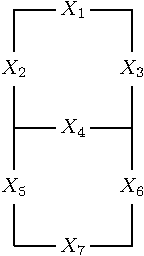
\includegraphics[]{figures/ch6_led.pdf}
    \caption{7-segment display}
    \label{fig:digits}
\end{figure}

Let us consider a seven-segment indicator displaying numerals using horizontal and
vertical lights in on-off combinations, as illustrated in
Figure~\ref{fig:digits}. Let $Y$ be a random variable taking its value in $\{0, 1,
..., 9\}$ with equal probability and  let $X_1, ..., X_7$ be binary variables
whose values are each determined univocally given the corresponding value of $Y$
in Table~\ref{table:digits}.

Since Table~\ref{table:digits} perfectly defines the data distribution, and
given the small dimensionality of the problem, it is practicable to directly
apply Equation~\ref{eqn:imp-full} to compute variable importances. To verify our
theoretical developments, we then compare in Table~\ref{table:imp} variable
importances as computed by Equation~\ref{eqn:imp-full} and those yielded by an
ensemble of $10000$ totally randomized trees ($K=1$). Note that given the  known
structure of the problem, building trees on a sample of finite size  that
perfectly follows the data distribution amounts to building them on a sample of
infinite size. At best, trees can thus be built on a 10-sample dataset,
containing exactly one sample for each of the equiprobable outcomes of $Y$. As
the table illustrates, the importances yielded by totally randomized trees match
those computed by Equation~\ref{eqn:imp-full}, which confirms
Theorem~\ref{thm:imp}. Small differences stem from the fact that a finite number
of  trees were built in our simulations, but those discrepancies should
disappear as the size of the ensemble grows towards infinity. It also shows that
importances indeed add up to $I(X_1, ... X_7;Y)$, which confirms
Theorem~\ref{thm:sum-of-imp}.
Regarding the actual importances, they indicate that $X_5$ is stronger than all
others, followed -- in that order -- by $X_2$, $X_4$ and $X_3$ which also show
large importances. $X_1$, $X_7$ and $X_6$ appear to be the less informative. The
table also reports importances for increasing values of $K$. As discussed before,
we see that a large value of $K$ yields importances that can be either
overestimated (e.g., at $K=7$, the importances of $X_2$ and $X_5$ are larger
than at $K=1$) or underestimated due to masking effects (e.g., at $K=7$, the
importances of $X_1$, $X_3$, $X_4$ and $X_6$ are smaller than at $K=1$, as if
they were less important). It can also be observed that masking effects may even
induce changes in the variable rankings (e.g., compare the rankings at $K=1$ and
at $K=7$), which thus confirms that importances are differently affected.

\begin{table}
    \centering
    \begin{tabular}{| c | c c c c c c c |}
    \hline
    $y$ & $x_1$ & $x_2$ & $x_3$ & $x_4$ & $x_5$ & $x_6$ & $x_7$ \\
    \hline
    \hline
    0 & 1 & 1 & 1 & 0 & 1 & 1 & 1 \\
    1 & 0 & 0 & 1 & 0 & 0 & 1 & 0 \\
    2 & 1 & 0 & 1 & 1 & 1 & 0 & 1 \\
    3 & 1 & 0 & 1 & 1 & 0 & 1 & 1 \\
    4 & 0 & 1 & 1 & 1 & 0 & 1 & 0 \\
    5 & 1 & 1 & 0 & 1 & 0 & 1 & 1 \\
    6 & 1 & 1 & 0 & 1 & 1 & 1 & 1 \\
    7 & 1 & 0 & 1 & 0 & 0 & 1 & 0 \\
    8 & 1 & 1 & 1 & 1 & 1 & 1 & 1 \\
    9 & 1 & 1 & 1 & 1 & 0 & 1 & 1 \\
    \hline
    \end{tabular}
    \caption{Values of $Y, X_1, ..., X_7$}
    \label{table:digits}
\end{table}

\begin{table}
    \begin{tabular}{| c | c c c c c c c c |}
    \hline
        & Eqn.~\ref{eqn:imp-full} & $K=1$ & $K=2$ & $K=3$ & $K=4$ & $K=5$ & $K=6$ & $K=7$ \\
    \hline
    \hline
    $X_1$ & 0.412 & 0.414 & 0.362 & 0.327 & 0.309 & 0.304 & 0.305 & 0.306\\
    $X_2$ & 0.581 & 0.583 & 0.663 & 0.715 & 0.757 & 0.787 & 0.801 & 0.799\\
    $X_3$ & 0.531 & 0.532 & 0.512 & 0.496 & 0.489 & 0.483 & 0.475 & 0.475\\
    $X_4$ & 0.542 & 0.543 & 0.525 & 0.484 & 0.445 & 0.414 & 0.409 & 0.412\\
    $X_5$ & 0.656 & 0.658 & 0.731 & 0.778 & 0.810 & 0.827 & 0.831 & 0.835\\
    $X_6$ & 0.225 & 0.221 & 0.140 & 0.126 & 0.122 & 0.122 & 0.121 & 0.120\\
    $X_7$ & 0.372 & 0.368 & 0.385 & 0.392 & 0.387 & 0.382 & 0.375 & 0.372\\
    \hline
    \hline
    $\sum$& 3.321 & 3.321 & 3.321 & 3.321 & 3.321 & 3.321 & 3.321 & 3.321\\
    \hline
    \end{tabular}
    \caption{Variable importances as computed with an ensemble of randomized trees, for increasing values of $K$. Importances at $K=1$ follow their theoretical values, as predicted by Equation~\ref{eqn:imp-full} in Theorem~\ref{thm:imp}. However, as $K$ increases,  importances diverge due to masking effects. In accordance with Theorem~\ref{thm:sum-of-imp}, their sum is also always equal to $I(X_{1}, \ldots, X_{7}; Y) = H(Y) = \log_{2}(10)= 3.321$ since inputs allow to perfectly predict the output.}
    \label{table:imp}
\end{table}

\begin{figure}
    \centering
    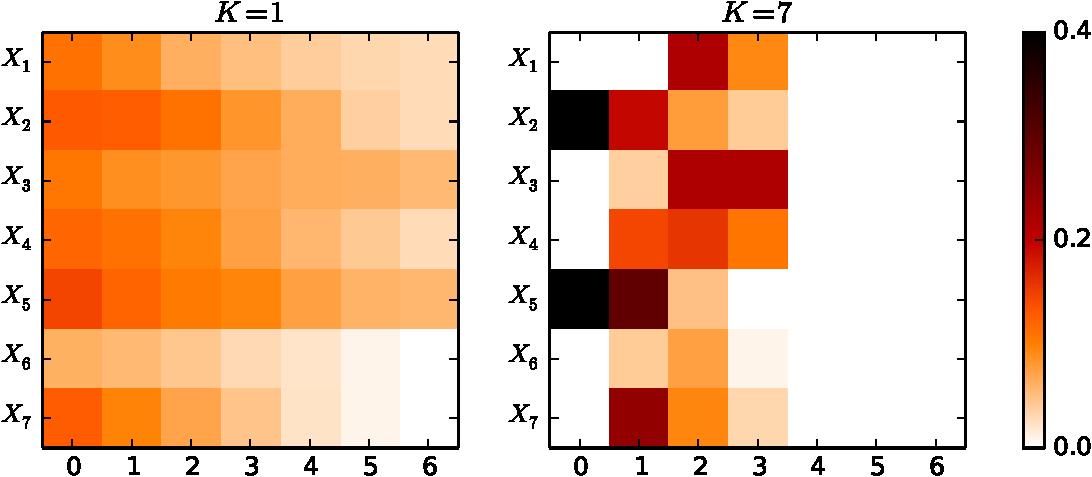
\includegraphics[width=0.9\textwidth]{figures/ch6_imp_led.pdf}
    \caption{Decomposition of variable importances along the degrees $k$ of interactions of one variable with the other ones. At $K=1$, all $I(X_j;Y|B)$ are accounted for in the total importance, while at $K=7$ only some of them are taken into account due to masking effects.}
    \label{fig:decomposition}
\end{figure}


To better understand why a variable is important, it is also insightful to look
at its decomposition into its $p$ sub-importances terms, as shown in
Figure~\ref{fig:decomposition}. Each row in the plots of the figure corresponds
to one the $p=7$ variables and each column to a size $k$ of conditioning sets.
As such, the value at row $m$ and column $k$ corresponds the importance of $X_j$
when conditioned with $k$ other variables (e.g., to the term $\frac{1}{C^k_p}
\frac{1}{p-k} \sum_{B \in {\cal P}_k(V^{-m})} I(X_j;Y|B)$ in Equation~\ref{eqn:imp-full}
in the case of totally randomized trees). In the left plot, for
$K=1$, the figure first illustrates how importances yielded by totally
randomized trees decomposes along the degrees $k$ of interactions terms. We can
observe that they each equally contribute (at most) the total importance of a
variable. The plot also illustrates why $X_5$ is important: it is informative
either alone or conditioned with any combination of the other variables (all of
its terms are significantly larger than $0$). By contrast, it also clearly shows
why $X_6$ is not important: neither alone nor combined with others $X_6$ seems
to be very informative (all of its terms are close to $0$). More interestingly,
this figure also highlights redundancies: $X_7$ is informative alone or
conditioned with a couple of others (the first terms are significantly larger
than $0$), but becomes uninformative  when conditioned with
many others (the last terms are closer to $0$). The right plot, for $K=7$,
illustrates the decomposition of importances when variables are chosen in a
deterministic way. The first thing to notice is masking effects. Some of the
$I(X_j;Y|B)$ terms are indeed clearly never encountered and their contribution
is therefore reduced to $0$ in the total importance. For instance, for $k=0$,
the sub-importances of $X_2$ and $X_5$ are positive, while all others are null,
which means that only those two variables are ever selected at the root node,
hence masking the others. As a consequence, this also means that the importances
of the remaining variables is biased and that it actually only accounts of their
relevance when conditioned to $X_2$ or $X_5$, but not of their relevance in
other contexts. At $k=0$, masking effects also amplify the contribution of $I(X_2;Y)$
(resp. $I(X_5;Y)$) since $X_2$ (resp. $X_5$) appears more frequently at the root
node than in totally randomized trees. In addition, because nodes become pure
before reaching depth $p$, conditioning sets of size $k\geq4$ are never actually
encountered, which means that we can no longer know whether variables are still
informative when conditioned to many others. All in all, this figure thus indeed
confirms that importances as computed with non-totally randomized trees take
into account only some of the conditioning sets $B$, hence biasing the measured
importances.


\section{Conclusions}

In this chapter, we made a first step towards understanding variable importances as
computed with a forest of randomized trees. In particular, we derived a
theoretical characterization of the Mean Decrease Impurity importances as
computed by totally randomized trees in asymptotic  conditions.  We showed that
they offer a three-level decomposition of the information jointly provided by
all input variables about the output (Section~\ref{sec:6:theory}). We then demonstrated
(Section~\ref{sec:6:variable-relevance}) that MDI importances as computed by totally randomized
trees exhibit desirable properties for  assessing the relevance of a variable:
it is equal to zero if and only if the variable is irrelevant and it depends
only on the relevant variables. We discussed the case of Random Forests and
Extra-Trees (Section~\ref{sec:6:variants}) and finally illustrated our
developments on an artificial but insightful example (Section~\ref{sec:6:illustration}).

There remain several limitations to our framework that we would like address in
the future. First, our results should be adapted to binary splits as used within
an actual Random Forest-like algorithm. In this setting, any node $t$ is split
in only two subsets, which means that any variable may then appear one or
several times within a branch, and thus should make variable importances now
dependent on the cardinalities of the input variables. In the same direction,
our framework should also be extended to the case of continuous variables.
Finally, results presented in this work are valid in an asymptotic setting only.
An important direction of future work includes the characterization of the
distribution of variable importances in a finite setting.
